\documentclass[11pt,openany]{article}

\usepackage{mathtools, commath}
% Packages for formatting
\usepackage[margin=1in]{geometry}
\usepackage{fancyhdr}
\usepackage{enumerate}
\usepackage{graphicx}
\usepackage{kotex}
\usepackage{arydshln} % Include this package
\usepackage{bbding}
\usepackage{amsmath}
\usepackage{amsthm}
\usepackage[dvipsnames,table]{xcolor}
\usepackage{amssymb, amsfonts}
\usepackage{wasysym}
\usepackage{footnote}
\usepackage{tablefootnote}
\usepackage{arydshln} % Include this package
% Fonts
\usepackage[T1]{fontenc}
\usepackage[utf8]{inputenc}
\usepackage{newpxtext,newpxmath}
\usepackage{sectsty}

% Define colors
\definecolor{TealBlue1}{HTML}{0077c2}
\definecolor{TealBlue2}{HTML}{00a5e6}
\definecolor{TealBlue3}{HTML}{b3e0ff}
\definecolor{TealBlue4}{HTML}{00293c}
\definecolor{TealBlue5}{HTML}{e6f7ff}

\definecolor{thmcolor}{RGB}{231, 76, 60}
\definecolor{defcolor}{RGB}{52, 152, 219}
\definecolor{lemcolor}{RGB}{155, 89, 182}
\definecolor{corcolor}{RGB}{46, 204, 113}
\definecolor{procolor}{RGB}{241, 196, 15}

\usepackage{color,soul}
\usepackage{soul}
\newcommand{\mathcolorbox}[2]{\colorbox{#1}{$\displaystyle #2$}}
\usepackage{cancel}
\newcommand\crossout[3][black]{\renewcommand\CancelColor{\color{#1}}\cancelto{#2}{#3}}
\newcommand\ncrossout[2][black]{\renewcommand\CancelColor{\color{#1}}\cancel{#2}}

\usepackage{hyperref}
\usepackage{booktabs}

% Chapter formatting
\definecolor{titleTealBlue}{RGB}{0,53,128}
\usepackage{titlesec}
\titleformat{\section}
{\normalfont\sffamily\Large\bfseries\color{titleTealBlue!100!gray}}{\thesection}{1em}{}
\titleformat{\subsection}
{\normalfont\sffamily\large\bfseries\color{titleTealBlue!50!gray}}{\thesubsection}{1em}{}

%Tcolorbox
\usepackage[most]{tcolorbox}
\usepackage{multirow}
\usepackage{multicol}

\usepackage[linesnumbered,ruled]{algorithm2e}
\usepackage{algpseudocode}
\usepackage{setspace}
\SetKwComment{Comment}{/* }{ */}
\SetKwProg{Fn}{Function}{:}{end}
\SetKw{End}{end}
\SetKw{DownTo}{downto}

% Define a new environment for algorithms without line numbers
\newenvironment{algorithm2}[1][]{
	% Save the current state of the algorithm counter
	\newcounter{tempCounter}
	\setcounter{tempCounter}{\value{algocf}}
	% redefine the algorithm numbering (remove prefix)
	\renewcommand{\thealgocf}{}
	\begin{algorithm}
	}{
	\end{algorithm}
	% Restore the algorithm counter state
	\setcounter{algocf}{\value{tempCounter}}
}

\usepackage{adjustbox}
% Header and footer formatting
\pagestyle{fancy}
\fancyhead{}
\fancyhf{}
\rhead{\textcolor{TealBlue2}{\large\textbf{기대수(기초부터 대학원 수학까지 시리즈) 3기}}}%\rule{3cm}{0.4pt}}
\lhead{\textcolor{TealBlue2}{\large\textbf{수학의 즐거움, Enjoying Math}}}
% Define footer
%\newcommand{\footer}[1]{
%\begin{flushright}
%	\vspace{2em}
%	\includegraphics[width=2.5cm]{school_logo.jpg} \\
%	\vspace{1em}
%	\textcolor{TealBlue2}{\small\textbf{#1}}
%\end{flushright}
%}
%\rfoot{\large Department of Information Security, Cryptogrphy and Mathematics, Kookmin Uni.\includegraphics[height=1.5cm]{school_logo.jpg}}
\fancyfoot{}
\fancyfoot[C]{-\thepage-}

\usepackage{tcolorbox}
\tcbset{colback=white, arc=5pt}

\definecolor{axiomcolor}{HTML}{a88bfa}
\definecolor{defcolor}{RGB}{52, 152, 219}
\definecolor{procolor}{RGB}{241, 196, 15}
\definecolor{thmcolor}{RGB}{231, 76, 60}
\definecolor{lemcolor}{RGB}{155, 89, 182}
\definecolor{corcolor}{RGB}{46, 204, 113}
\definecolor{execolor}{RGB}{90, 128, 127}

% Define a new command for the custom tcolorbox
\newcommand{\axiombox}[2][]{%
	\begin{tcolorbox}[colframe=axiomcolor, title={\color{white}\bfseries #1}]
		#2
	\end{tcolorbox}
}

\newcommand{\defbox}[2][]{%
	\begin{tcolorbox}[colframe=defcolor, title={\color{white}\bfseries #1}]
		#2
	\end{tcolorbox}
}

\newcommand{\lembox}[2][]{%
	\begin{tcolorbox}[colframe=lemcolor, title={\color{white}\bfseries #1}]
		#2
	\end{tcolorbox}
}

\newcommand{\probox}[2][]{%
	\begin{tcolorbox}[colframe=procolor, title={\color{white}\bfseries #1}]
		#2
	\end{tcolorbox}
}

\newcommand{\thmbox}[2][]{%
	\begin{tcolorbox}[colframe=thmcolor, title={\color{white}\bfseries #1}]
		#2
	\end{tcolorbox}
}

\newcommand{\corbox}[2][]{%
	\begin{tcolorbox}[colframe=corcolor, title={\color{white}\bfseries #1}]
		#2
	\end{tcolorbox}
}



\usepackage{amsthm}

% Define custom theorem styles
\newtheoremstyle{dotless} % Name of the style
{3pt} % Space above
{3pt} % Space below
{\itshape} % Body font
{} % Indent amount
{\bfseries} % Theorem head font
{} % Punctuation after theorem head
{2.5mm} % Space after theorem head
{} % Theorem head spec

\newtheoremstyle{definitionstyle} % Name of the style
{3pt} % Space above
{3pt} % Space below
{} % Body font
{} % Indent amount
{\bfseries} % Theorem head font
{.} % Punctuation after theorem head
{2.5mm} % Space after theorem head
{} % Theorem head spec

% Applying custom styles
\theoremstyle{dotless}
\newtheorem{theorem}{Theorem} % Theorem environment with section-wise numbering
\newtheorem{proposition}[theorem]{Proposition} % Theorem environment with section-wise numbering
\newtheorem{lemma}[theorem]{Lemma} % Lemma shares the counter with theorem
\newtheorem{corollary}[theorem]{Corollary} % Corollary shares the counter with theorem

\theoremstyle{definitionstyle}
\newtheorem*{observation}{\textcolor{Magenta}{Observation}}
\newtheorem{definition}{Definition} % Definition shares the counter with theorem
\newtheorem{example}{Example} % Example shares the counter with theorem
\newtheorem{exercise}{Exercise} % Example shares the counter with theorem
\newtheorem{remark}{Remark} % Remark shares the counter with theorem
\newtheorem*{note}{Note}

\newtheorem*{definition*}{Definition} % Definition shares the counter with theorem
\newtheorem*{example*}{Example} % Example shares the counter with theorem
\newtheorem*{exercise*}{\textcolor{violet}{Exercise}} % Example shares the counter with theorem
\newtheorem*{remark*}{Remark} % Remark shares the counter with theorem


\usepackage{tikz}
\usepackage{tikz-cd}
\usepackage{tikz-3dplot}
\usepackage{pgfplots}
\pgfplotsset{compat=newest} % Adjust to your version of pgfplots
\def\Circlearrowleft{\ensuremath{%
		\rotatebox[origin=c]{180}{$\circlearrowleft$}}}
\def\Circlearrowright{\ensuremath{%
		\rotatebox[origin=c]{180}{$\circlearrowright$}}}
\def\CircleArrowleft{\ensuremath{%
		\reflectbox{\rotatebox[origin=c]{180}{$\circlearrowleft$}}}}
\def\CircleArrowright{\ensuremath{%
		\reflectbox{\rotatebox[origin=c]{180}{$\circlearrowright$}}}}
\usetikzlibrary{
	3d, % For 3D drawing
	angles,
	arrows,
	arrows.meta,
	backgrounds,
	bending,
	calc,
	decorations.pathmorphing,
	decorations.pathreplacing,
	decorations.markings,
	fit,
	matrix,
	patterns,
	patterns.meta,
	positioning,
	quotes,
	shadows,
	shapes,
	shapes.geometric,
	tikzmark
}
\tikzset{
	% single mid‐path arrow
	mid arrow/.style={
		decoration={
			markings,
			mark=at position 0.5 with {\arrow{Stealth[scale=1.2]}}
		},
		postaction={decorate},
	},
	% style for field arrows
	field arrow/.style={
		-{Stealth[scale=1.0]},
		thick,
		blue!70!black,
	},
}
\newcommand{\ie}{\textnormal{i.e.}}
\newcommand{\rsa}{\mathsf{RSA}}
\newcommand{\rsacrt}{\mathsf{RSA}\textendash\mathsf{CRT}}
\newcommand{\inv}[1]{#1^{-1}}

%New Command
%\newcommand{\set}[1]{\left\{#1\right\}}
\newcommand{\N}{\mathbb{N}}
\newcommand{\Z}{\mathbb{Z}}
\newcommand{\Q}{\mathbb{Q}}
\newcommand{\R}{\mathbb{R}}
\newcommand{\cR}{\mathcal{R}}
\newcommand{\C}{\mathbb{C}}
\newcommand{\F}{\mathbb{F}}
\newcommand{\nbhd}{\mathcal{N}}
\newcommand{\Log}{\operatorname{Log}}
\newcommand{\Arg}{\operatorname{Arg}}
\newcommand{\pv}{\operatorname{P.V.}}

\newcommand{\of}[1]{\left( #1 \right)} 
%\newcommand{\abs}[1]{\left\lvert #1 \right\rvert}
%\newcommand{\norm}[1]{\left\| #1 \right\|}

\newcommand{\sol}{\textcolor{magenta}{\bf Sol}}
\newcommand{\conjugate}[1]{\overline{#1}}

\newcommand{\res}{\operatorname{res}}
\DeclareMathOperator*{\Res}{\operatorname{Res}}

%\renewcommand{\Re}{\operatorname{Re}}
%\renewcommand{\Im}{\operatorname{Im}}

\newcommand{\cyclic}[1]{\langle #1 \rangle}
\newcommand{\uniform}{\overset{\$}{\leftarrow}}
\newcommand{\xmark}{\textcolor{red}{\XSolidBrush}}
\newcommand{\vmark}{\textcolor{green!75!black}{\CheckmarkBold}}

\newcommand{\gen}[1]{\langle #1 \rangle}
\newcommand{\Gen}[1]{\left\langle #1 \right\rangle}

\newcommand{\img}[1]{\text{Img}(#1)}
\newcommand{\Img}[1]{\text{Img}\left(#1\right)}
\newcommand{\preimg}[1]{\text{Img}^{-1}(#1)}
\newcommand{\Preimg}[1]{\text{Img}^{-1}\left(#1\right)}

\newcommand{\relation}{\mathrel{\mathcal{R}}}
\newcommand{\injection}{\rightarrowtail}
\newcommand{\surjection}{\twoheadrightarrow}
\newcommand{\id}{\textnormal{id}}

\newcommand{\eqclass}[1]{\left[#1\right]}

% Define custom colors for O and X
\newcommand{\yes}{\textcolor{blue}{\bf \fullmoon}}
\newcommand{\no}{\textcolor{red}{\bf \texttimes}}

\DeclarePairedDelimiter\ceil{\lceil}{\rceil}
\DeclarePairedDelimiter\floor{\lfloor}{\rfloor}
%\renewcommand{\floor}[#1]{\lfloor #1\rfloor}
%\newcommand{\Floor}[#1]{\left\lfloor #1\right\rfloor}
%\newcommand{\ceil}[#1]{\lceil #1\rceil}
%\newcommand{\Ceil}[#1]{\left\lceil #1\right\rceil}

\newcommand{\topology}{\mathscr{T}}
\newcommand{\sequence}[1]{\langle #1\rangle}

\setstretch{1.25}
\begin{document}
\pagenumbering{arabic}
\begin{center}
	\huge\textbf{Set Theory II}\\
	\vspace{0.5em}
	\large{Ji, Yong-hyeon}\\
	\vspace{0.5em}
	\normalsize{\today}\\
\end{center}

\noindent We cover the following topics in this note.
\begin{itemize}
	\item Relations
	\item Equivalence Relations
	\item Equivalence Classes
	\item Partitions
\end{itemize}
\hrule\vspace{12pt}
\defbox[Relation]{\begin{definition*}
	Let $A\times B$ be the cartesian product of two sets $A$ and $B$. A \hl{(\textbf{binary}) \textbf{relation}} on $A\times B$ is a subset  $\mathcal{R}$ of $A\times B$. That is, \[
	\mathcal{R}\ \text{is a relation on}\ A\times B\iff \mathcal{R}\subseteq A\times B.
	\]
\end{definition*}}
\begin{remark*}
	$\mathcal{R}$ is a relation on $A$ $\iff$ $\mathcal{R}\subseteq A\times A$.
\end{remark*}
\begin{note}[Notation]
	Let $(s,t)\in\mathcal{R}$. We use the notation $s\relation t$ and we can say ``\textbf{$s$ is related to $t$ by $R$}''. If $(s,t)\notin\mathcal{R}$, we denote as: $s\centernot\relation t$.
\end{note}
\vfill
\begin{example*}
	Let $A=\set{1,2}$ and $B=\set{4,5}$. Then \[
	A\times B=\set{(1,4),(1,5),(2,4),(2,5)}.
	\] Here, $\mathcal{R}=\set{(1,4),(2,5)}\subseteq A\times B$ be a relation.
	\begin{center}
	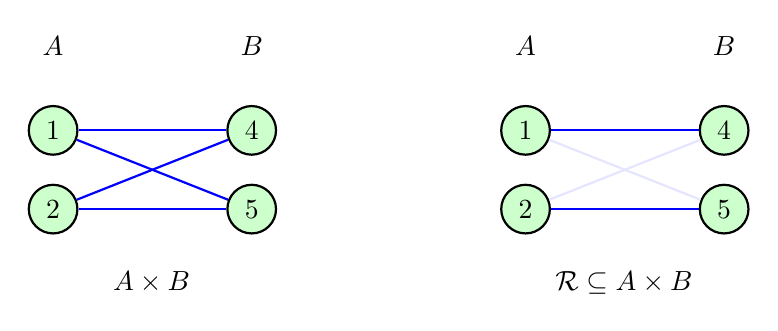
\begin{tikzpicture}[>=Stealth, node distance=1cm and 2cm]
	\tikzset{
		set node/.style={rectangle, draw, thick, fill=orange!20, minimum size=5mm, align=center},
		relation arrow/.style={-, thick, #1},
		element node/.style={circle, draw, thick, fill=green!20, minimum size=5mm},
		highlight/.style={draw, thick, dotted, inner sep=3pt}
	}
	
	% Define nodes for elements
	\node[] (a) {$A$};
	\node[right=of a] (b) {$B$};
	\node[element node, below=0.5cm of a] (1) {1};
	\node[element node, below of=1] (2) {2};
	\node[element node, below=0.5cm of b] (4) {4};
	\node[element node, below of=4] (5) {5};
	
	\foreach \x in {1, 2} {
		\draw[relation arrow=blue] (\x) -- (4);
		\draw[relation arrow=blue] (\x) -- (5);
	}

	\node at (1.25,-3) {$A\times B$};
	\begin{scope}[xshift=6cm]
		\node[] (a) {$A$};
		\node[right=of a] (b) {$B$};
		\node[element node, below=0.5cm of a] (1) {1};
		\node[element node, below of=1] (2) {2};
		\node[element node, below=0.5cm of b] (4) {4};
		\node[element node, below of=4] (5) {5};
		
		\draw[relation arrow=blue] (1) -- (4);
		\draw[relation arrow=blue!10] (1) -- (5);
		\draw[relation arrow=blue!10] (2) -- (4);
		\draw[relation arrow=blue] (2) -- (5);
		
		\node at (1.25,-3) {$\mathcal{R}\subseteq A\times B$};
	\end{scope}
\end{tikzpicture}

	\end{center}
\end{example*}

\begin{example*}
	Let $A$ and $B$ are sets, and let $f:A\to B$ be a function form $A$ to $B$. Then \[
	(a,b)\in f\iff a\mathrel{f}b\iff b=f(a).
	\]
\end{example*}

\newpage
\defbox[$\star$ Equivalence Relation $\star$]{\begin{definition*}
	A binary relation $\mathcal{R}$ on a set $S$ is called an \hl{\textbf{equivalence relation}} if it satisfies the following three properties: for all $a,b,c\in S$,
	\begin{enumerate}[(i)]
		\item (Reflexivity) $(a,a)\in\mathcal{R}$;
		\item (Symmetry) $(a,b)\in\mathcal{R}\implies(b,a)\in\mathcal{R}$;
		\item (Transitivity) $(a,b)\in\mathcal{R}\land (b,c)\in\mathcal{R}\implies(a,c)\in\mathcal{R}$.
	\end{enumerate}
\end{definition*}}
\begin{remark*}
	\ \begin{figure}[h!]\centering
	\adjustbox{scale=.9}{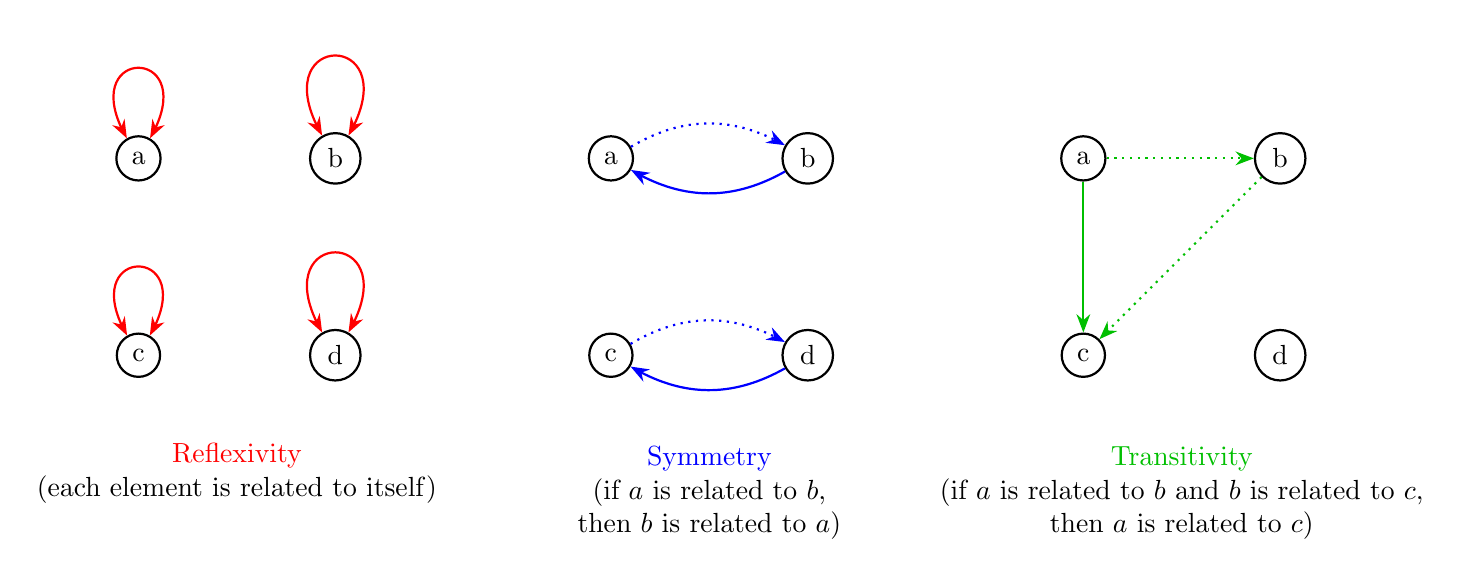
\begin{tikzpicture}[>=Stealth, node distance=2.5cm, thick, main/.style = {draw, circle}]
	% Define styles
	\tikzset{
		reflexive/.style={<->, loop, looseness=12, in=120, out=60, red},
		symmetric/.style={->, blue, bend left},
		transitive/.style={->, green!75!black}
	}
	
	% Nodes
	\node[main] (a) {a};
	\node[main] (b) [right of=a] {b};
	\node[main] (c) [below of=a] {c};
	\node[main] (d) [right of=c] {d};
	
	% Edges
	% Reflexivity
	\draw[reflexive] (a) to (a);
	\draw[reflexive] (b) to (b);
	\draw[reflexive] (c) to (c);
	\draw[reflexive] (d) to (d);
	\begin{scope}[xshift=6cm]
		% Nodes
		\node[main] (a2) {a};
		\node[main] (b2) [right of=a2] {b};
		\node[main] (c2) [below of=a2] {c};
		\node[main] (d2) [right of=c2] {d};
		
		% Symmetry
		\draw[dotted,symmetric] (a2) to (b2);
		\draw[symmetric] (b2) to (a2);
		\draw[dotted,symmetric] (c2) to (d2);
		\draw[symmetric] (d2) to (c2);
	\end{scope}
	
	\begin{scope}[xshift=12cm]
		% Nodes
		\node[main] (a3) {a};
		\node[main] (b3) [right of=a3] {b};
		\node[main] (c3) [below of=a3] {c};
		\node[main] (d3) [right of=c3] {d};
		
		% Transitivity
		\draw[dotted, transitive] (a3) to (b3);
		\draw[dotted, transitive] (b3) to (c3);
		\draw[transitive] (a3) to (c3); % Transitivity implied by a -> d and d -> b
	\end{scope}
	
	\node[align=center] at (1.25,-4) {\textcolor{red}{Reflexivity}\\ (each element is related to itself)};
	\node[align=center] at (7.25,-4.25) {\textcolor{blue}{Symmetry}\\ (if \(a\) is related to \(b\),\\ then \(b\) is related to \(a\))};
	\node[align=center] at (13.25,-4.25) {\textcolor{green!75!black}{Transitivity}\\ (if \(a\) is related to \(b\) and \(b\) is related to \(c\),\\ then \(a\) is related to \(c\))};
	
	% Annotations
%	\node[align=left, below right= of c] {
%		%		\textbf{Equivalence Relation Properties:}\\
%		\textcolor{red}{Red arrows: Reflexivity}\\ (each element is related to itself).\\
%		\textcolor{blue}{Blue arrows: Symmetry}\\ (if \(a\) is related to \(b\), then \(b\) is related to \(a\)).\\
%		\textcolor{green}{Green arrows: Transitivity}\\ (if \(a\) is related to \(b\) and \(b\) is related to \(c\), then \(a\) is related to \(c\)).
%	};
\end{tikzpicture}}
	\end{figure}
\end{remark*}
\vfill
\begin{example*}
	Let $A=\set{1,2,3,4}$. Then \begin{align*}
		\mathcal{R}=\{\textcolor{red}{(1,1)},\textcolor{red}{(2,2)},\textcolor{red}{(3,3)},\textcolor{red}{(4,4)},\textcolor{gray}{(1,2)},\textcolor{gray}{(2,1)}\}
	\end{align*} is an equivalence relation on $A$.
	\begin{figure}[h!]\centering
		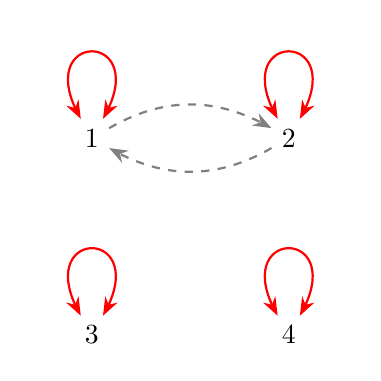
\begin{tikzpicture}[>=Stealth, node distance=2.5cm, thick, main/.style = {draw, circle}]
	% Define styles
	\tikzset{
		reflexive/.style={<->, loop, looseness=12, in=120, out=60, red},
		symmetric/.style={->, blue, bend left},
		transitive/.style={->, green!75!black}
	}
	
%	\draw[rounded corners=25pt] (-1,2) rectangle (3.5,-3);
	
	% Nodes
	\node[] (a) {1};
	\node[] (b) [right of=a] {2};
	\node[] (c) [below of=a] {3};
	\node[] (d) [right of=c] {4};
	
	% Edges
	% Reflexivity
	\draw[reflexive] (a) to (a);
	\draw[reflexive] (b) to (b);
	\draw[reflexive] (c) to (c);
	\draw[reflexive] (d) to (d);
	
	\draw[->, dashed, gray, bend left] (a) to (b);
	\draw[->, dashed, gray, bend left] (b) to (a);
\end{tikzpicture}
	\end{figure}
\end{example*}

\newpage
%\begin{note}[Notation]
%	Let $A$ and $B$ are sets, and let $f:A\to B$ is a function from $A$ to $B$. \begin{enumerate}[(1)]
%		\item 
%	\end{enumerate}
%\end{note}
\begin{note}
	Let $A,B,C$ are sets, and let $f:A\to B$ and $g:B\to C$ are functions.
	\begin{itemize}
		\item We claim that $\boxed{(g\circ f)[A]=g[f[A]]}$:\[
		(g\circ f)[A]=\set{(g\circ f)(a):a\in A}=\set{g(f(a)):a\in A}=\set{g(b):b=f(a)\in f[A]}=g[f[A]].
		\]
		\item We claim that $\boxed{f\ \text{is surjective}\iff \img{f}=f[A]=B}$: \[
			f:A\twoheadrightarrow B\iff \forall b\in B,\ \exists a\in A\ \text{s.t.}\ f(a)=b\iff f[A]=\set{f(a)\in B:a\in A}=B.
			\]
	\end{itemize} 
\end{note}
\lembox{\begin{lemma}\hypertarget{lemma1}{}
	Let $A,B$ and $C$ are sets, and let $f:A\to B$ and $g:B\to C$ are functions.
	\begin{enumerate}[(1)]
		\item If $f$ and $g$ are both one-to-one, then $(g\circ f):A\to C$ is one-to-one.
		\item If $f$ and $g$ are both onto, then $(g\circ f):A\to C$ is onto.
	\end{enumerate}
\end{lemma}}
\begin{proof}
	\textcolor{gray!30!white}{\begin{enumerate}[(1)]
		\item Let $f$ and $g$ are both one-to-one. We must show that $(g\circ f):A\to C$ is one-to-one. Suppose that $(g\circ f)(a)=(g\circ f)(a')$. Then \begin{align*}
			(g\circ f)(a)=(g\circ f)(a') &\implies g(f(a))=g(f(a')) &\text{by def. of composition} \\&\implies f(a)=f(a') &\because\text{$g$ is injective} \\
			&\implies a=a'. &\because\text{$f$ is injective}
		\end{align*}
		\item Let $f$ and $g$ are both onto. We must show that $(g\circ f):A\to C$ is onto, \ie, $(g\circ f)[A]=C$.
		\begin{align*}
			(g\circ f)[A] &=g[f[A]] \\
			&= g[B] &\because\text{$f:A\to B$ is surjective, \ie, $f[A]=B$} \\
			&= C. &\because\text{$g:B\to C$ is surjective, \ie, $g[B]=C$} \\
		\end{align*}
	\end{enumerate}}
\end{proof}
\lembox{\begin{lemma}\hypertarget{lemma2}{}
	Let $A,B$ and $C$ are sets, and let $f:A\to B$ and $g:B\to C$ are functions. \begin{enumerate}[(1)]
		\item If $(g\circ f):A\to C$ is one-to-one, then $f$ is one-to-one.
		\item If $(g\circ f):A\to C$ is onto, then $g$ is onto.
	\end{enumerate}
\end{lemma}}
\begin{proof}
\textcolor{gray!30!white}{\begin{enumerate}[(1)]
	\item Let $g\circ f$ is one-to-one. We must show that $f$ is one-to-one. Suppose that $f(a)=f(a')$. Then \begin{align*}
		f(a)=f(a') &\implies g(f(a))=g(f(a')) &\because\text{$g$ is a function} \\
		&\implies(g\circ f)(a)=(g\circ f)(a')&\text{by the def. of composition} \\
		&\implies a=a'.&\because\text{$g\circ f$ is injective}
	\end{align*}
	\item Let $g\circ f$ is onto, \ie, $(g\circ f)[A]=C$. We must show that $g$ is onto, \ie, $g[B]=C$:
	\begin{itemize}
		\item[($\subseteq$)] $g[B]=\set{g(b)\in C: b\in B}\subseteq C$;
		\item[($\supseteq$)] $C=(g\circ f)[A]=g[f[A]]=\set{g(b)\in C:b\in f[A]}\subseteq g[B]$.
	\end{itemize}
\end{enumerate}}
\end{proof}
\vfill
\probox[Equivalence Relation on $2^A$ Based on Bijection]{\begin{proposition}
	Let $A$ be a set, and $2^A$ be its power set. Define a relation $\mathcal{R}$ on $2^A$ as follows: \[
	X\sim_{\mathcal{R}} Y\iff \exists (f:X\to Y)\ \text{such that $f$ is bijective},
	\] for $X,Y\in 2^A$. In other words, \[
	\mathcal{R}:=\set{(X,Y)\in 2^A\times 2^A:\exists\ \text{a bijection}\ (f:X\to Y)}.
	\]
\end{proposition}}
\begin{proof}
	Let $X,Y,Z\in 2^A$. We must show that $\sim_{\mathcal{R}}$ is reflexive, symmetric and transitive: 
	\begin{enumerate}[(i)]
		\item (Reflexivity) We NTS\footnote{`NTS` means that ``need to show``.} that $X\sim_{\mathcal{R}} X$. In other words, we need to find a bijection from $X$ it self. 
		\begin{center}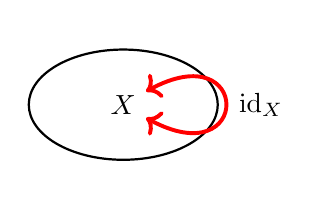
\begin{tikzpicture}[scale=1, every node/.style={scale=1}]
			% Reflexivity
			\draw[thick] (0, 0) ellipse (1.2 and 0.7) node[text=black] (X) {$X$};
			\draw[<->, loop, looseness=12, in=30, out=-30, line width=.5mm, red] (X) to (X);
			\node at (1.75,0) {$\text{id}_X$};
		\end{tikzpicture}\end{center}
		Consider the identity function \[
		\fullfunction{\text{id}_X}{X}{X}{x}{x=\text{id}_X(x)}
		\] for all $x\in X$. Clearly, $\id_X$ is a bijection. Thus, $X\sim_{\mathcal{R}} X$.
		\vfill
		\item (Symmetry) We NTS that $X\sim_{\mathcal{R}} Y\implies Y\sim_{\mathcal{R}} X$. In other words, if there exists a bijection $f:X\to Y$, then there must exists a bijection $g:Y\to X$. 
		\begin{center}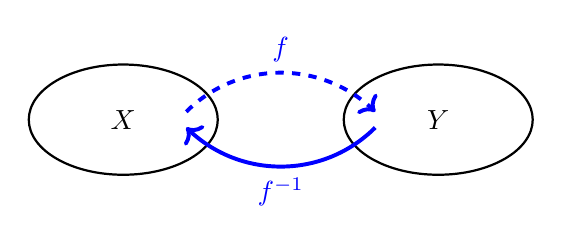
\begin{tikzpicture}[scale=1, every node/.style={scale=1}]
		\draw[thick] (0, 2.5) ellipse (1.2 and 0.7) node[text=black] {$X$};
		\draw[thick] (4, 2.5) ellipse (1.2 and 0.7) node[text=black] {$Y$};
		
		\draw[->, thick, dashed, line width=.5mm, blue] (0.8, 2.6) to[out=45, in=135] node[above] {$f$} (3.2, 2.6);
		\draw[->, thick, line width=.5mm, blue] (3.2, 2.4) to[out=225, in=315] node[below] {$f^{-1}$} (0.8, 2.4);
		\end{tikzpicture}\end{center}
		Suppose that $f:X\to Y$ is a bijection. Then it has an inverse function $f^{-1}:Y\to X$, which satisfies: \[
		\forall x\in X:f^{-1}(f(x))=x=\id_X(x)\quad\text{and}\quad \forall y\in X:f(f^{-1}(y))=y=\id_Y(y).
		\] That is, $f^{-1}\circ f=\id_X$ and $f\circ f^{-1}=\id_Y$. By \hyperlink{lemma2}{\textbf{Lemma 2}}, $f^{-1}$ must be a bijection since $f$, $\id_X$ and $\id_Y$ are bijections. Thus, there is a bijection $g=f^{-1}$.
		\vfill
		\item We NTS that $X\sim_{\mathcal{R}}Y\land Y\sim_{\mathcal{R}} Z\implies X\sim_{\mathcal{R}} Z$. In other words, if there exists two bijection $f:X\to Y$ and $g:Y\to Z$, then there must exists a bijection $h:X\to Z$.
		\begin{center}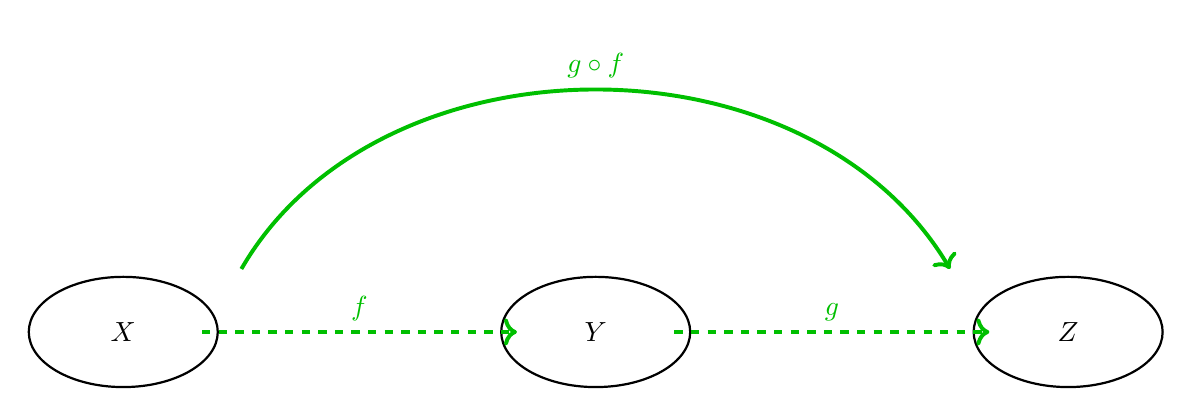
\begin{tikzpicture}[scale=1, every node/.style={scale=1}]
		\draw[thick] (-6, -2) ellipse (1.2 and 0.7) node[text=black] {$X$};
		\draw[thick] (0, -2) ellipse (1.2 and 0.7) node[text=black] {$Y$};
		\draw[thick] (6, -2) ellipse (1.2 and 0.7) node[text=black] {$Z$};
		
		\draw[->, thick, dashed, line width=.5mm, green!75!black] (-5, -2) to node[above] {$f$} (-1, -2);
		\draw[->, thick, dashed, line width=.5mm, green!75!black] (1, -2) to node[above] {$g$} (5, -2);
		\draw[->, thick, line width=.5mm, green!75!black] (-4.5, -1.2) to[out=60, in=120] node[above] {$g \circ f$} (4.5, -1.2);
		\end{tikzpicture}\end{center}
		Suppose that $f:X\to Y$ and $g:Y\to Z$ both are bijective. Define the function \[
		\fullfunction{h}{X}{Z}{x}{(g\circ f)(x)=h(x)}
		\] for all $x\in X$. By \hyperlink{lemma1}{\textbf{Lemma 1}}, $h=g\circ f$ must be a bijection since $f$ and $g$ are both bijective.
	\end{enumerate}
	Hence it is proved.
\end{proof}

\newpage
\defbox[Indexed Family]{\begin{definition*}
	Let $I$ and $S$ are sets. Consider a function $A:I\to S$ defined by $i\mapsto A(i)=:A_i$. The image $\img{A}$ is called an \textbf{\hl{indexed family} of elements in $S$ indexed by $I$}. We write this indexed family as: \[
	\Gen{A_i}_{i\in I}.
	\] Note that \[
	\img{A}=\set{A(i):i\in I}=\set{A_i:i\in I}=\Gen{A_i}_{i\in I}.
	\]
\end{definition*}}
\begin{example*}[Sequence]
	Let $I=\N$ be an indexing set. Then \[
	S:=\set{A_1,A_2,A_3,A_4,\cdots}=\set{A_i:i\in\N}=\gen{A_i}_{i\in\mathbb{N}}
	\] is an indexed family of elements in $S$ indexed by $\mathbb{N}$.
\end{example*}
\vspace{50pt}
\defbox[Union and Intersection of an Indexed Family]{\begin{definition*}
	Let $I$ and $S$ are sets, and let $\Gen{A_i}_{i\in}$ be an indexed family in $S$. \begin{itemize}
		\item The \textbf{union} of $\Gen{A_i}_{i\in}$ is defined by \[
		\bigcup_{i\in I}A_i:=\set{x\in S:\exists i\in I\ \text{such that}\ x\in A_i}.
		\] 
		\item The \textbf{intersection} of $\Gen{A_i}_{i\in}$ is defined by \[
		\bigcap_{i\in I}A_i:=\set{x\in X:\forall i\in I,\ x\in A_i}.
		\]
	\end{itemize}
\end{definition*}}
\begin{remark*}
	Let $I=\set{1,\dots,n}$. Then \begin{itemize}
		\item $\displaystyle\bigcup_{i\in I}S_i=\bigcup_{i=1}^nS_i=S_1\cup S_2\cup\cdots\cup S_n$.
		\item $\displaystyle\bigcap_{i\in I}S_i=\bigcap_{i=1}^nS_i=S_1\cap S_2\cap\cdots\cap S_n$.
	\end{itemize}
\end{remark*}

\newpage
\defbox[$\star$ Partitions $\star$]{\begin{definition*}
	Let $S$ be a set. Let $\gen{A_i}_{i\in I}$ be a family of subsets of $S$, where $A_i\subseteq S$ for each index $i\in I$. The family $\Gen{A_i}_{i\in I}$ is called a \textbf{\hl{partition} of $S$} if the following conditions hold:
	\begin{enumerate}[(i)]
		\item (\textbf{Non-empty Subsets}) $A_i\neq\varnothing$ for all $i\in I$. Formally \[
		\boxed{\forall i\in I,\ A_i\neq\varnothing}.
		\]
		\item (\textbf{Pairwise Disjoint}) For any $i,j\in I$, if $i\neq j$, then $A_i\cap A_j=\varnothing$. Formally \[
		\boxed{\forall i,j\in I,\ \left[i\neq j\implies A_i\cap A_j=\varnothing\right]}.
		\]
		\item (\textbf{Union Covers the Whole Set}) The union of all sets $A_i$ is the whole set $S$. Formally \[
		\boxed{\bigcup_{i\in A}A_i=S}.
		\]
	\end{enumerate}
\end{definition*}}

\begin{example*}
	Let $\mathbb{Z}$ be a set of integers. We define an indexed family $\Gen{A_i}_{i\in\set{0,1,2}}$ of subsets of $\mathbb{Z}$ as follows: \begin{align*}
		A_0=\set{n\in\mathbb{Z}: n\equiv 0\ (\bmod 3)}=\set{n\in\mathbb{Z}:n=3k+0\ \text{for some}\ k\in\mathbb{Z}}=:[0],\\
		A_1=\set{n\in\mathbb{Z}: n\equiv 1\ (\bmod 3)}=\set{n\in\mathbb{Z}:n=3k+1\ \text{for some}\ k\in\mathbb{Z}}=:[1],\\
		A_2=\set{n\in\mathbb{Z}: n\equiv 2\ (\bmod 3)}=\set{n\in\mathbb{Z}:n=3k+2\ \text{for some}\ k\in\mathbb{Z}}=:[2].
	\end{align*}
\begin{minipage}{.5\textwidth}
Then \begin{enumerate}[(i)]
	\item $[0]\neq\varnothing$, $[1]\neq\varnothing$ and $[2]\neq\varnothing$.
	\item \begin{align*}
		[0]\cap[1] &= \varnothing, \\
		[1]\cap[2] &= \varnothing, \\
		[2]\cap[0] &= \varnothing.
	\end{align*}
	\item $[0]\cup [1]\cup [2]=\mathbb{Z}$.
\end{enumerate} Thus, \[
\set{A_1,A_2,A_3}=\set{[0],[1],[2]}
\]is a partition of $\mathbb{Z}$.
\end{minipage}
\begin{minipage}{.5\textwidth}
\adjustbox{scale=.65,center}{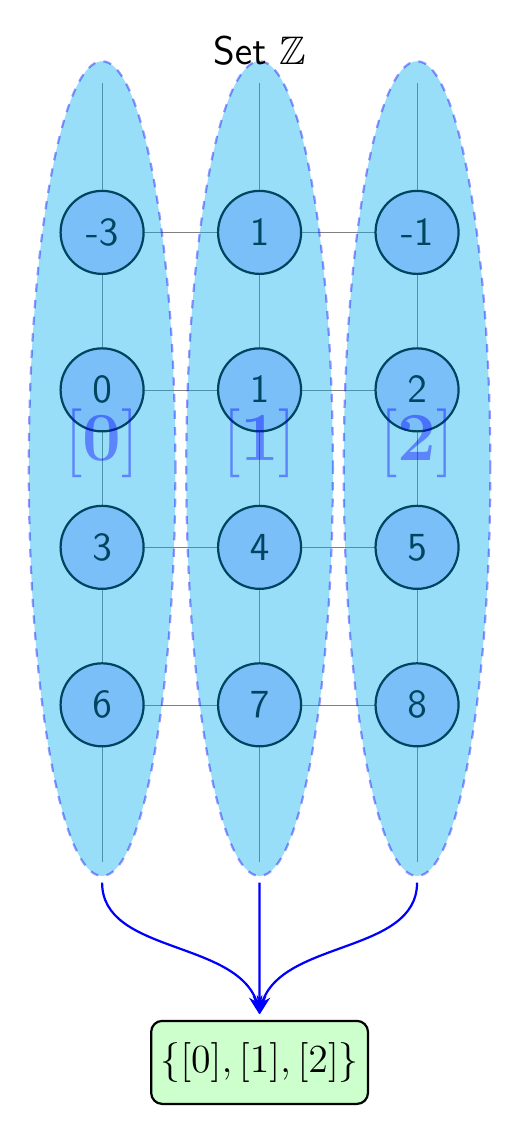
\begin{tikzpicture}[>=Stealth, thick, node distance=2cm, auto]
	% Styles
	\tikzset{
		main node/.style={circle, draw, fill=blue!20, minimum size=30pt, font=\sffamily\Large},
		class node/.style={dashed, ellipse, draw, thick, blue, fill=cyan, minimum height=1cm, minimum width=1cm, align=center, opacity=.4}, % drop shadow
		quotient node/.style={rectangle, draw, thick, fill=green!20, minimum size=30pt, font=\sffamily\Large, rounded corners},
		path/.style={blue,-Stealth, thick, shorten <=2pt, shorten >=2pt, decorate},
		%decoration={snake, amplitude=.4mm, segment length=2mm, post length=1mm}
		label distance=2mm
	}
	
	% Nodes representing elements of the set% Nodes representing elements
	
	\node[main node] (0) {0};
	\node[main node] (1) [right of=0] {1};
	\node[main node] (2) [right of=1] {2};
	
	\node[main node] (-3) [above of=0] {-3};
	\node[main node] (-2) [above of=1] {1};
	\node[main node] (-1) [above of=2] {-1};
	
	\node[main node] (3) [below of=0] {3};
	\node[main node] (4) [below of=1] {4};
	\node[main node] (5) [below of=2] {5};
	
	\node[main node] (6) [below of=3] {6};
	\node[main node] (7) [below of=4] {7};
	\node[main node] (8) [below of=5] {8};
	
	% Nodes for equivalence classes
	\node[class node, fit=(-3) (0) (6)] (class0) {\Huge $\mathbf{[0]}$};
	\node[class node, fit=(-2) (1) (7)] (class1) {\Huge $\mathbf{[1]}$};
	\node[class node, fit=(-1) (2) (8)] (class2) {\Huge $\mathbf{[2]}$};
	
	% Quotient set nodes
	\node[quotient node, below=4cm of $(6)!0.5!(8)$] (qset) {$\{[0], [1], [2]\}$};
	
	% Paths for quotient set formation
	\draw[path] (class0) to[out=-90, in=90] (qset);
	\draw[path] (class1) to[out=-90, in=90] (qset);
	\draw[path] (class2) to[out=-90, in=90] (qset);
	
	% Annotations and decorative lines
	\node[align=center, above=2cm of $(-3)!0.5!(-1)$, font=\sffamily\Large] {Set $\Z$};
%	\node[align=center, below=0.5cm of qset, font=\sffamily\Large] {Quotient Set $\Z/5\Z$};
	
	% Background grid
	\begin{scope}[on background layer]
		\draw[style=help lines, step=2cm, gray, very thin] (0,3.9) grid (4,-6);
	\end{scope}
\end{tikzpicture}
}
\end{minipage}
\end{example*}

\newpage
\defbox[$\star$ Equivalence Class $\star$]{\begin{definition*}
	Let $\cR\subseteq S\times S$ be an equivalence relation on $S$. The \textbf{\hl{equivalence class} of $x\in S$ under $\cR$} is the set \[
	\eqclass{x}_{\cR}=\set{y\in S:x\relation y}.
	\]
\end{definition*}}
\begin{note}
	Note that $\alpha\relation x\iff \alpha\in[x]_{\mathcal{R}}\iff x\relation \alpha$.
\end{note}
\lembox[]{\begin{lemma}
	Let $\mathcal{R}$ be an equivalence relation on a set $S$. For any $x, y \in S$, let $\eqclass{x}$ and $[y]$ represent the equivalence classes of $x$ and $y$, respectively, under $\mathcal{R}$.
	\begin{enumerate}[(1)]
		\item \hypertarget{lemma-4-1}{$\forall x\in S,\ x\in\eqclass{x}$}.
		\item \hypertarget{lemma-4-2}{$x\relation y\iff \eqclass{x}=[y]$}.
		\item \hypertarget{lemma-4-3}{$x\centernot\relation y\iff \eqclass{x}\cap [y]=\varnothing$}.
	\end{enumerate}
\end{lemma}}
\begin{proof}
	\textcolor{gray!30!white}{\begin{enumerate}[(1)]
		\item Let $x\in S$. Since $\cR$ is reflexive, we have $x\relation x$, \ie, $x\in\eqclass{x}$.
		\item \begin{itemize}
			\item[$(\Rightarrow)$] Let $x\relation y$. We NTS that $[x]=[y]$: \begin{itemize}
				\item[$(\subseteq)$] Let $\alpha\in\eqclass{x}$, \ie, $\alpha\relation x$. Then 
				\begin{align*}
					\alpha\relation x&\implies \alpha\relation y&\because\text{$x\relation y$ and $\cR$ is transitive} \\
					&\implies \alpha\in[y].
				\end{align*}
				\item[$(\supseteq)$] Let $\beta\in[y]$, \ie, $y\relation\beta$. Then 
				\begin{align*}
					y\relation\beta&\implies x\relation \beta&\because\text{$x\relation y$ and $\cR$ is transitive} \\
					&\implies \beta\in[x].
				\end{align*}
			\end{itemize}
			\item[$(\Leftarrow)$] Let $[x]=[y]$. Then $
			x\in S\overset{\text{by (1)}}{\implies} x\in[x]=[y]\implies x\in[y]\implies x\relation y.$
		\end{itemize}
		\item \begin{itemize}
			\item[$(\Rightarrow)$] Let $x\centernot\relation y$. Suppose that $\eqclass{x}\cap[y]\neq\varnothing$ then $\exists \gamma\in S$ such that $\gamma\in\eqclass{x}\cap[y]$. Then \begin{align*}
				\gamma\in [x]\cap [y]\implies \gamma\in [x]\land\gamma\in [y]\implies x\relation\gamma\land \gamma\relation y\implies x\relation y\ \text{\LARGE\lightning}.
			\end{align*}
			\item[$(\Leftarrow)$] Let $\eqclass{x}\cap[y]=\varnothing$. Suppose that $x\relation y$. By (1) and (2), we have $x\in[x]=[y]\ \text{\LARGE\lightning}$.
		\end{itemize}
	\end{enumerate}}
\end{proof}
\thmbox[]{\begin{theorem}
	Let $S$ be a set and let $\mathcal{R}$ be an equivalence relation on $S$. Define the set of equivalence classes \[
	\mathcal{P}:=\set{[x]_{\mathcal{R}}:x\in S},
	\] where $[x]_{\mathcal{R}}=\set{y\in S:x\relation y}$. Then $\mathcal{P}$ forms a partition of $S$.
\end{theorem}}
\begin{proof}
	We must show that the set of equivalence classes $\set{[x]_{\mathcal{R}}:x\in S}$ satisfies the three conditions of a partition:
	\begin{enumerate}[(i)]
		\item (Equivalence Class is not Empty) By \hyperlink{lemma-4-1}{(1) of \textbf{Lemma 4}}, it is proved.
		\item (Equivalence Classes are Disjoint) By \hyperlink{lemma-4-2}{(2) and (3) of \textbf{Lemma 4}}, it is proved.
		\item (Union of Equivalence Classes is Whole Set) We NTS that $\displaystyle\bigcup\set{[x]_{\mathcal{R}}:x\in S}=S$:
		\begin{itemize}
			\item[($\subseteq$)] Since $[x]_{\mathcal{R}}\subseteq S$, we have \begin{align*}
				\bigcup\set{[x]_{\mathcal{R}}:x\in S}=\bigcup_{x\in S}[x]_{\mathcal{R}}\subseteq S.
			\end{align*}
			\item[($\supseteq$)] Let $\alpha\in S$. We want to show that $\displaystyle\alpha\in\bigcup_{x\in S}[x]_{\mathcal{R}}$, \ie, \[
			\exists x\in S\ \text{such that}\ \alpha\in[x].
			\]
		\end{itemize} By \hyperlink{lemma-4-1}{(1) of \textbf{Lemma 4}}, we obtain $\alpha\in[\alpha]$. Thus, for every $\alpha\in S$, $\displaystyle\alpha\in\bigcup_{x\in S}[x]_{\mathcal{R}}$.
	\end{enumerate}
\end{proof}

\newpage
\thmbox[]{\begin{theorem}
	Let $S$ be a set and $\mathcal{P}=\Gen{P_i}_{i\in I}$ be a partition of $S$. We define a relation ${\mathcal{R}}$ on $S$: \[
	x\sim_{\mathcal{R}}y \iff \exists i\in I\ \text{such that}\ x,y\in P_i
	\] for all $x,y\in S$. That is, $x$ is related to $y$ under $\mathcal{R}$ if and only if $x$ and $y$ belong to the same subset $P_i$ in the partition. Then $\mathcal{R}$ is the equivalence relation induced by a partition $\mathcal{P}$.
\end{theorem}}
\begin{proof}
	\textcolor{gray!30!white}{Let $\Gen{P_i}_{i\in I}$ be a partition of $S$. That is, \[
	\text{(a)}\ P_i\neq\varnothing\ \text{for all}\ i\in I;\hspace{30pt}
	\text{(b)}\ P_i\cap P_j=\varnothing\ \text{for}\ i\neq j;\hspace{30pt}
	\text{(c)}\ \bigcup_{i\in I}P_i=S.
	\]
	Let $x,y\in S$. Note that \[
	\mathcal{R}:=\set{(x,y)\in S\times S: \exists i\in I\ \text{s.t.}\ x\in P_i\land y\in P_i}.
	\]We NTS $\sim_{\mathcal{R}}$ is reflexive, symmetric and transitive:
	\begin{enumerate}[(i)]
		\item (Reflexivity) We NTS that $x\sim_{\mathcal{R}} x$: \[
		x\in S\overset{\text{by (c)}}{\implies} x\in \bigcup_{i\in I}P_i\implies \exists i\in I\ \text{s.t.}\ x\in P_i\implies \exists i\in I\ \text{s.t.}\ x\in P_i\land x\in P_i\implies x\sim_{\mathcal{R}} x.
		\]
		\item (Symmetry) We NTS that $x\sim_{\mathcal{R}} y\implies y\sim_{\mathcal{R}} x$:\[
		x\sim_{\mathcal{R}} y\implies \exists i\in I\ \text{s.t.}\ x\in P_i\land y\in P_i\implies \exists i\in I\ \text{s.t.}\ y\in P_i\land x\in P_i\implies y\sim_{\mathcal{R}} x.
		\]
		\item (Transitivity) We NTS that $x\sim_{\mathcal{R}} y\land y\sim_{\mathcal{R}} z\implies x\sim_{\mathcal{R}} z$:\[
		\begin{cases*}
			x\sim_{\mathcal{R}} y \\
			y\sim_{\mathcal{R}} z
		\end{cases*}\implies \begin{cases*}
		\exists i\in I\ \text{s.t.}\ x\in P_i\land \underline{y\in P_i} \\
		\exists j\in I\ \text{s.t.}\ \underline{y\in P_j}\land z\in P_j
	\end{cases*}\overset{\text{by (b), $i=j$}}{\implies}\exists i=j\in I\ \text{s.t.}\ x\in P_i\land z\in P_i\implies x\sim_{\mathcal{R}} z.
		\]
	\end{enumerate}}
\end{proof}

%\thmbox[$\star\star\star$ Fundamental Theorem of Equivalence Relation $\star\star\star$]{\begin{theorem}
%	
%\end{theorem}}



\vfill
\begin{thebibliography}{9}
	\bibitem{set_thery_c}
	수학의 즐거움, Enjoying Math. ``수학 공부, 기초부터 대학원 수학까지, 3. 집합론 기초 (c).'' YouTube Video, 35:04. Published 
	September 07, 2019. URL: \url{https://www.youtube.com/watch?v=2gM-Vh8CY8I&list=PL4m4z_pFWq2pLwFsWf0KJX_uMNo-jktN5&index=136}.
\end{thebibliography}

\end{document}
